\documentclass[11pt, a4paper]{article}


\usepackage{tocbibind}
\usepackage{makeidx}
\usepackage[utf8]{inputenc}
\usepackage{chngcntr}
\usepackage{verbatim}
\usepackage{csquotes}
\usepackage{soul}
\usepackage{booktabs}
\usepackage{graphicx}
\usepackage[spanish]{babel}
\usepackage[bottom=0.5cm]{geometry}
\usepackage{floatrow}
\usepackage{colortbl}
\usepackage[table]{xcolor}
\usepackage{longtable}
\usepackage{vmargin}
\usepackage{parskip}
\usepackage{changepage}
\usepackage{setspace}
\usepackage{lipsum}
\usepackage{changepage}
\usepackage{fancyhdr}
\usepackage[T1]{fontenc}
\usepackage{array}
\usepackage{booktabs}
\usepackage{ragged2e}
\usepackage{amsmath}
\usepackage{times}
\usepackage{mathptmx}
\usepackage{parskip}
\usepackage{rotating}
\usepackage{adjustbox}
\usepackage{caption}
\usepackage{array}
\usepackage{multirow}
\usepackage{graphicx}
\usepackage{titlesec}
\usepackage{tabularx}

\usepackage{tikz}
\usetikzlibrary{shapes.geometric, arrows}



\titleclass{\subsubsubsection}{straight}[\subsection]
\newcounter{subsubsubsection}
\renewcommand\thesubsubsubsection{\thesubsubsection.\arabic{subsubsubsection}}
\titleformat{\subsubsubsection}
  {\normalfont\normalsize\bfseries}{\thesubsubsubsection}{1em}{}
\titlespacing*{\subsubsubsection}
  {0pt}{3.25ex plus 1ex minus .2ex}{1.5ex plus .2ex}

\setcounter{secnumdepth}{4}
\setcounter{tocdepth}{4}


\counterwithin{table}{section}  % Reinicia el contador de tablas en cada sección
\counterwithin{figure}{section}  
\fancyhf{} % Limpia todos los encabezados y pies de página predeterminados

\captionsetup[table]{name=Tabla}
\renewcommand{\listtablename}{Índice de tablas}


% Definir el color personalizado
\definecolor{cabecera_tabla}{RGB}{71, 106, 133}
\definecolor{fila_gris}{RGB}{242, 242, 242}
\definecolor{fila_verde}{RGB}{235, 241, 221}
\definecolor{borde_tabla}{RGB}{221, 221, 221}

\newlength{\halfbaselineskip}
\setlength{\halfbaselineskip}{0.5\baselineskip}

\ifPDFTeX
  \usepackage[T1]{fontenc}
  \usepackage[utf8]{inputenc}
  \usepackage{textcomp}
\else
  \usepackage{unicode-math}
  \defaultfontfeatures{Scale=MatchLowercase}
  \defaultfontfeatures[\rmfamily]{Ligatures=TeX,Scale=1}
\fi

\IfFileExists{upquote.sty}{\usepackage{upquote}}{}
\IfFileExists{microtype.sty}{
  \usepackage[]{microtype}
  \UseMicrotypeSet[protrusion]{basicmath}
}{}

\makeatletter
\@ifundefined{KOMAClassName}{
  \IfFileExists{parskip.sty}{
    \usepackage{parskip}
  }{
    \setlength{\parindent}{0pt}
    \setlength{\parskip}{6pt plus 2pt minus 1pt}
  }
}{
  \KOMAoptions{parskip=half}
}
\makeatother

\usepackage{xcolor}
\IfFileExists{xurl.sty}{\usepackage{xurl}}{}
\IfFileExists{bookmark.sty}{\usepackage{bookmark}}{\usepackage{hyperref}}
\hypersetup{
  hidelinks,
  linktoc=all
}
\urlstyle{same}

\usepackage{longtable,booktabs,array}
\usepackage{calc}
\usepackage{etoolbox}
\makeatletter
\patchcmd\longtable{\par}{\if@noskipsec\mbox{}\fi\par}{}{}
\makeatother

\usepackage{fancyhdr}
\pagestyle{fancy}


\addto\captionsspanish{
  \renewcommand{\listtablename}{Índice de tablas}
}


% Encabezado superior
\fancyhead[R]{\small TERMOFLUIDODINÁMICA}
\fancyhead[R]{\small Trabajo Combustión}
% Aplicar el encabezado solo en la primera página
% Pie de página inferior
\fancyfoot[C]{\small Paula Domínguez Morales - UAX}


\begin{document}
%\begin{spacing}{1.2} % Espaciado de 1 líneas
\begin{quote}
\begin{center}
%\begin{spacing}{1.2} % Espaciado de 1 líneas

\setlength{\parskip}{12pt} % Aumenta el espacio vertical entre párrafos

%\setlength{\headheight}{13.6pt}
%\addtolength{\topmargin}{-1.6pt}

\begin{adjustwidth}{-1.7cm}{-1cm}
\begin{quote}
\begin{center}
\begin{spacing}{1.2} % Espaciado de 1 líneas


\setlength{\parskip}{8pt} % Aumenta el espacio vertical entre párrafos
\vspace*{1cm} % Agrega un espacio vertical antes de la imagen
\begin{center}

\includegraphics[width=4.209424in,height=2.805199507in]{media/image1.png}
\end{center}

\thispagestyle{empty}
\vspace{1.3cm} % Agrega un espacio vertical de 1 cm
{\fontsize{17}{20}\selectfont UNIVERSIDAD ALFONSO X EL SABIO}

\vspace{1cm} % Agrega un espacio vertical de 0.7 cm
{\fontsize{17}{20}\selectfont Máster Universitario en Ingeniería Aeronáutica}

\vspace{1cm} % Agrega un espacio vertical de 1 cm
{\fontsize{18}{20}\selectfont\textbf{TERMOFLUIDODINÁMICA}}

\vspace{1cm} % Agrega un espacio vertical de 1 cm


{\fontsize{18}{20}\selectfont\textbf{Trabajo Combustión}}

\vspace{2cm} % Agrega un espacio vertical de 1 cm

Autor: Paula Domínguez Morales (855681)

Fecha: 20-Enero-25
\end{spacing} 
\end{center}
\end{quote}
\end{adjustwidth}

%\newpage{\ }


\begin{adjustwidth}{-1.7cm}{-1cm}


\begin{quote}
\setlength{\parskip}{1pt} % Aumenta el espacio vertical entre párrafos
\vspace*{0.5cm} % Agrega un espacio vertical antes de la imagen
\begin{center}
{\fontsize{18}{20}\selectfont\textbf{Lista de abreviaturas}}
\end{center}
\end{quote}
\vspace*{1cm} % Agrega un espacio vertical de 1 cm

{\fontsize{14}{20}\selectfont\textbf{Abreviaturas}}
\vspace{0.2cm} % Agrega un espacio vertical de 1 cm
{\setstretch{2}

\begin{itemize}
    \item \textbf{CH$_4$}: Metano
    \item \textbf{CO$_2$}: Dióxido de carbono
    \item \textbf{H$_2$O}: Agua
    \item \textbf{O$_2$}: Oxígeno
    \item \textbf{phi}: Relación de equivalencia del combustible (dosado)
    \item \textbf{T}: Temperatura
    \item \textbf{P}: Presión
    \item \textbf{NM}: Millas náuticas
    \item \textbf{Et}: Eficiencia térmica
    \item \textbf{A}: Área del cambiador de calor
    \item \textbf{V/m}: Voltios por Metro
\end{itemize}
}

\vspace{1cm} % Agrega un espacio vertical de 1 cm



\newpage
\tableofcontents
% Suprimir las entradas del índice para Figuras y Tablas solo en la primera vez
\addtocontents{toc}{\protect\setcounter{tocdepth}{-1}}

% Restaurar la profundidad del índice después de imprimir los índices de figuras y tablas
\addtocontents{toc}{\protect\setcounter{tocdepth}{2}}

\newpage
\vspace*{0.05cm}
\listoffigures


\newpage
\vspace*{0.05cm}
\listoftables

\newpage

\begin{quote}
\setlength{\parskip}{1pt} % Aumenta el espacio vertical entre párrafos
\vspace*{0.3cm} % Agrega un espacio vertical antes de la imagen
\hypertarget{introducciuxf3n}{%
\section{INTRODUCCIÓN}\label{introducciuxf3n}}
\end{quote}
\vspace*{1cm} % Agrega un espacio vertical de 1 cm


Este documento aborda el diseño y análisis de una caldera basada en oxicombustión de metano para su aplicación en plantas de cogeneración. Se pretende estudiar tanto las condiciones de arranque inicial como los modos estacionarios de funcionamiento, evaluando aspectos clave del diseño y la operación.

El análisis incluye el cálculo de parámetros esenciales como la temperatura del quemador, la recirculación de gases, y la eficiencia térmica en diferentes configuraciones. También se identifican los posibles ajustes necesarios para optimizar el rendimiento y se analizan las limitaciones asociadas al diseño actual.

Además, se presta especial atención a la evaluación de los modos de operación propuestos, considerando sus ventajas y desventajas en términos de eficiencia y sostenibilidad. Este trabajo busca aportar una visión técnica detallada para el desarrollo de sistemas más eficientes y respetuosos con el medio ambiente, aprovechando las capacidades del metano como combustible en procesos industriales.


\vspace*{1cm}

\begin{figure}[h!]
\centering
 \includegraphics[width=6.86625209424in, height=2.60805199507in]{media/caldera.jpg}
\caption{Esquema del sistema de la caldera  \protect\hyperlink{bibliografia}{{[}1{]}}.}
\label{fig:caldera}
\end{figure}


\newpage

\begin{quote}
\setlength{\parskip}{1pt} % Aumenta el espacio vertical entre párrafos
\vspace*{0.3cm} % Agrega un espacio vertical antes de la imagen
\hypertarget{objetivos}{%
\section{OBJETIVOS}\label{objetivos}}
\end{quote}
\vspace*{1cm} % Agrega un espacio vertical de 1 cm


El objetivo principal de este trabajo es analizar el diseño y funcionamiento de una caldera de oxicombustión de metano en plantas de cogeneración, con el fin de optimizar su rendimiento y evaluar su viabilidad técnica. Para alcanzar este objetivo general, se plantean los siguientes objetivos específicos:

\begin{itemize}
    \item Determinar las condiciones necesarias para un arranque seguro, incluyendo el cálculo de la temperatura del quemador y las condiciones de ignición.
    \item Analizar las configuraciones de operación estacionaria, evaluando la recirculación de gases y su impacto en la eficiencia térmica.
    \item Calcular los parámetros clave de diseño, como el área del cambiador de calor y la longitud de la llama en distintos escenarios.
    \item Comparar las ventajas y desventajas de las configuraciones operativas propuestas (modo con condensador activado y modo sin condensador).
    \item Identificar limitaciones y oportunidades de mejora en el diseño actual, con especial atención a la reducción de emisiones y el aumento de la eficiencia energética.
\end{itemize}

Con estos objetivos se busca ofrecer una base técnica sólida para la optimización de sistemas de oxicombustión en aplicaciones industriales, considerando tanto los aspectos operativos como los ambientales.


\newpage

\begin{quote}
\setlength{\parskip}{1pt} % Aumenta el espacio vertical entre párrafos
\vspace*{0.3cm} % Agrega un espacio vertical antes de la imagen
\hypertarget{libyentorno}{%
\section{LIBRERIAS Y PREPARACIÓN DEL ENTORNO}\label{libyentorno}}
\end{quote}
\vspace*{1cm} % Agrega un espacio vertical de 1 cm

Para realizar este análisis, se utilizó Python como entorno principal debido a su flexibilidad y la disponibilidad de librerías específicas que permiten manejar modelos termodinámicos y cálculos de combustión. 

Entre las herramientas más destacadas, se incluyen librerías para cálculos matemáticos, manipulación de datos tabulares, creación de gráficos y, lo más importante, el modelado termodinámico de gases ideales y procesos de combustión. Estas herramientas se configuraron para proporcionar resultados precisos y reproducibles en el contexto del estudio de una caldera de oxicombustión de metano.

El modelo de gas ideal empleado permite definir propiedades específicas del aire, como su capacidad calorífica y la entalpía específica, las cuales son fundamentales para realizar cálculos de energía. Asimismo, se incluyó un modelo detallado para la simulación de la combustión, lo que permitió obtener valores precisos de la temperatura del quemador y la composición de los productos generados.

Gracias a la preparación adecuada del entorno, se obtuvieron resultados como:
\begin{itemize}
    \item La caracterización de las propiedades del aire y el metano para su uso en los cálculos.
    \item La posibilidad de realizar ajustes precisos en las condiciones iniciales de temperatura y presión para evaluar diferentes escenarios.
    \item La implementación de cálculos que integran herramientas termodinámicas avanzadas para analizar el comportamiento de los gases en condiciones de oxicombustión.
\end{itemize}

Este enfoque no solo garantiza la precisión de los resultados obtenidos, sino que también permite extender el análisis a escenarios adicionales en futuras investigaciones. La configuración del entorno y la selección de herramientas fueron pasos esenciales para establecer las bases del análisis.




\newpage

\begin{quote}
\setlength{\parskip}{1pt} % Aumenta el espacio vertical entre párrafos
\vspace*{0.3cm} % Agrega un espacio vertical antes de la imagen
\hypertarget{datos}{%
\section{DATOS Y PROPIEDADES DEL GAS }\label{datos}}
\end{quote}
\vspace*{1cm} % Agrega un espacio vertical de 1 cm


Para realizar el análisis de la oxicombustión de metano, se definieron cuidadosamente las propiedades iniciales del gas y sus condiciones operativas. Estos parámetros son esenciales para establecer el marco del análisis termodinámico y garantizar que los cálculos reflejen con precisión el comportamiento real de la caldera. 

A continuación, se detallan los principales parámetros utilizados:

\begin{itemize}
    \item \textbf{Composición del gas:} Se asumió una mezcla formada por metano (\textbf{CH$_4$}) como combustible y oxígeno (\textbf{O$_2$}) como comburente. Esta mezcla es característica de los procesos de oxicombustión, ya que optimiza la eficiencia al minimizar la presencia de nitrógeno en el sistema.
    \item \textbf{Relación estequiométrica:} Se definió una operación cercana al régimen estequiométrico, que garantiza un balance preciso entre la cantidad de combustible y de comburente. Este enfoque es fundamental para minimizar los residuos y maximizar la eficiencia térmica.
    \item \textbf{Condiciones iniciales:} 
    \begin{itemize}
        \item \textbf{Presión:} La presión de operación se estableció en 1 atmósfera, una condición estándar para muchos procesos de combustión.
        \item \textbf{Temperatura:} La temperatura inicial se fijó en 25°C (298 K), representando condiciones típicas de arranque.
    \end{itemize}
    \item \textbf{Propiedades termodinámicas:} Se calcularon magnitudes como la capacidad calorífica específica (\textit{c$_p$}) y la entalpía específica del aire, utilizando el modelo \texttt{SemiperfectIdealGas}. Este modelo, basado en una mezcla de gases ideales, permite representar con precisión las propiedades del aire y su influencia en los procesos de combustión.
\end{itemize}

Estos datos iniciales fueron empleados en diversos cálculos, entre ellos:
\begin{itemize}
    \item La estimación de la temperatura teórica alcanzada en el quemador durante la combustión.
    \item El análisis de las configuraciones de recirculación de gases en las etapas estacionarias de operación.
    \item La evaluación del rendimiento térmico del sistema bajo diferentes escenarios operativos.
\end{itemize}

Gracias a la precisión de los datos y las herramientas empleadas, se estableció una base sólida para modelar el comportamiento termodinámico del sistema y evaluar posibles ajustes en el diseño de la caldera. Este enfoque permitió realizar un análisis completo, con resultados aplicables tanto a condiciones reales como a estudios futuros.



\newpage



\begin{quote}
\setlength{\parskip}{1pt} % Aumenta el espacio vertical entre párrafos
\vspace*{0.3cm} % Agrega un espacio vertical antes de la imagen
\hypertarget{arranque}{%
\section{CONDICIÓN DE ARRANQUE}\label{arranque}}
\end{quote}
\vspace*{1cm} % Agrega un espacio vertical de 1 cm


\subsection*{1. Temperatura teórica durante el arranque}

El análisis del arranque de la caldera incluye la estimación de la temperatura teórica alcanzada en el quemador para diferentes relaciones de dosado (\(\phi\)), considerando escenarios de mezcla pobre (\(\phi < 1\)) y mezcla rica (\(\phi > 1\)). Estos cálculos permiten identificar el comportamiento térmico del sistema y optimizar el rendimiento inicial.

A continuación, se presentan los resultados obtenidos:

\begin{table}[h!]
\centering
\begin{tabular}{|c|c|}
\hline
\textbf{Dosado (\(\phi\))} & \textbf{Temperatura (K)} \\ \hline
0.1                        & 1014.47                 \\ \hline
0.5                        & 2202.07                 \\ \hline
0.9                        & 3693.29                 \\ \hline
1.1                        & 4479.60                 \\ \hline
1.5                        & 3912.56                 \\ \hline
2.0                        & 3728.28                 \\ \hline
\end{tabular}
\caption{Temperatura teórica durante el arranque en función del dosado (\(\phi\)).}
\label{tab:temperatura_dosado}
\end{table}

\vspace*{1cm}

\begin{figure}[h!]
\centering
 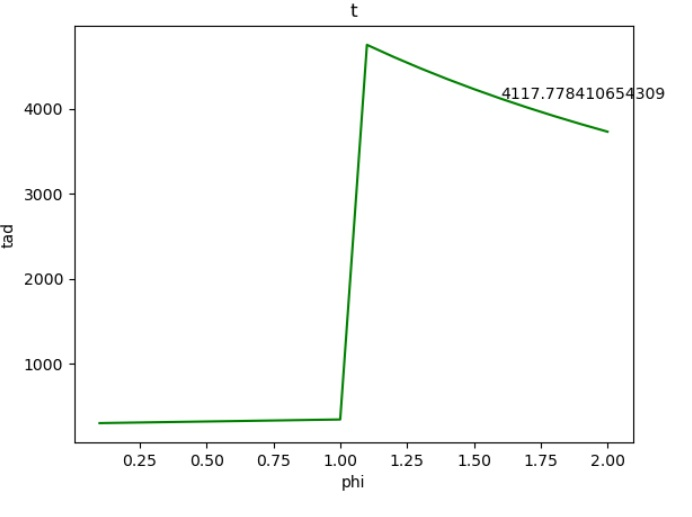
\includegraphics[width=4.486625209424in, height=3.360805199507in]{media/Tad_Caldera.jpg}
\caption{Temperatura adiabática de la Caldera.}
\label{fig:caldera}
\end{figure}

\newpage

\paragraph{Interpretación:}
La temperatura teórica máxima se alcanza cerca del dosado estequiométrico (\(\phi \approx 1\)), con un valor de aproximadamente \(4479.6 \, \text{K}\). En mezclas pobres, la temperatura incrementa a medida que se aproxima al dosado estequiométrico. En mezclas ricas, la temperatura disminuye debido al exceso de combustible no quemado.

Estos resultados destacan la importancia de operar cerca del dosado estequiométrico para maximizar la eficiencia térmica del sistema durante el arranque.


\subsection*{2. Metano inquemado durante el arranque}

En este apartado se evaluó la fracción de metano (\(\text{CH}_4\)) que no se quema por completo durante el arranque en función de la relación de dosado (\(\phi\)). Este análisis es fundamental para comprender la eficiencia del sistema y minimizar los residuos.

A continuación, se presentan los resultados obtenidos:

\begin{table}[h!]
\centering
\begin{tabular}{|c|c|c|c|}
\hline
\textbf{Dosado (\(\phi\))} & \textbf{Moles de CH$_4$ inyectados} & \textbf{Moles de CH$_4$ quemados} & \textbf{Moles de CH$_4$ no quemados} \\ \hline
1.0                        & 1.000                               & 1.000                            & 0.000                              \\ \hline
1.2                        & 1.200                               & 1.000                            & 0.200                              \\ \hline
1.4                        & 1.400                               & 1.000                            & 0.400                              \\ \hline
\end{tabular}
\caption{Moles de metano inyectado, quemado y no quemado según \(\phi\).}
\label{tab:metano_inquemado}
\end{table}

\paragraph{Interpretación:}
Para una relación de dosado estequiométrico (\(\phi = 1.0\)), todo el metano inyectado se quema, maximizando la eficiencia del sistema. Sin embargo, en mezclas ricas (\(\phi > 1.0\)), el exceso de metano no se quema, lo que resulta en una pérdida de eficiencia. Por ejemplo:
\begin{itemize}
    \item Con \(\phi = 1.2\), aproximadamente el \(16.7\%\) del metano inyectado queda sin quemar.
    \item Con \(\phi = 1.4\), este valor aumenta al \(28.6\%\).
\end{itemize}

\paragraph{Conclusión:}
Operar en condiciones cercanas al dosado estequiométrico (\(\phi \approx 1.0\)) es esencial para minimizar las emisiones de metano no quemado y optimizar la eficiencia térmica de la caldera.


\subsection*{3. Parámetros iniciales}

El arranque de la caldera se realizó bajo condiciones controladas, definiendo parámetros iniciales clave que afectan directamente al proceso de combustión. Estos parámetros incluyen:

\begin{itemize}
    \item \textbf{Presión inicial:} \(P = 1 \, \text{atm}\) (presión atmosférica estándar).
    \item \textbf{Temperatura inicial:} \(T = 298 \, \text{K}\) (25°C).
    \item \textbf{Volumen del quemador:} \(V_{\text{caldera}} = 0.0036 \, \text{m}^3\).
    \item \textbf{Relación estequiométrica:} Mezcla inicial ajustada a \(\phi = 1.0\) (dosado estequiométrico).
\end{itemize}

Estos valores garantizan condiciones estables de operación durante el arranque. La relación estequiométrica seleccionada maximiza la eficiencia térmica, mientras que la presión y temperatura iniciales se alinean con estándares operativos comunes.

\subsection*{4. Estimación de la longitud de llama}

Durante el arranque, la longitud de la llama se calculó considerando la velocidad de inyección del flujo y el tiempo de reacción. La longitud de llama (\(L_f\)) es un parámetro esencial para evaluar la estabilidad y seguridad del proceso. Su valor se obtiene mediante la expresión:

\[
L_f = V_{\text{caldera}} \cdot v_{\text{inyección}} \cdot t_{\text{reacción}}
\]

Donde:
\begin{itemize}
    \item \(V_{\text{caldera}} = 0.0036 \, \text{m}^3\) es el volumen de la caldera.
    \item \(v_{\text{inyección}} = 6.25 \, \text{m/s}\) es la velocidad de inyección.
    \item \(t_{\text{reacción}} = 0.04 \, \text{s}\) es el tiempo necesario para completar la reacción de combustión.
\end{itemize}

Sustituyendo estos valores, se obtiene:
\[
L_f = 0.0036 \cdot 6.25 \cdot 0.04 = 0.009 \, \text{m}
\]

\paragraph{Interpretación:}
La longitud de llama estimada es de \(9 \, \text{mm}\). Este valor sugiere un proceso de combustión estable y controlado, ideal para el arranque seguro del sistema.

\subsection*{5. Velocidad de inyección y tiempo de reacción}

El análisis del arranque incluye el cálculo de dos parámetros fundamentales: la velocidad de inyección y el tiempo de reacción.

\paragraph{Velocidad de inyección:}
La velocidad de inyección (\(v_{\text{inyección}}\)) se calcula como:
\[
v_{\text{inyección}} = \frac{\dot{V}_{\text{caldera}}}{A_{\text{caldera}}}
\]

Donde:
\begin{itemize}
    \item \(\dot{V}_{\text{caldera}} = 0.0225 \, \text{m}^3/\text{s}\) es el caudal volumétrico.
    \item \(A_{\text{caldera}} = \frac{\pi \cdot d^2}{4}\) es el área de la caldera, con \(d = 0.1 \, \text{m}\) (diámetro).
\end{itemize}

Sustituyendo, se obtiene:
\[
A_{\text{caldera}} = \frac{\pi \cdot (0.1)^2}{4} = 0.00785 \, \text{m}^2
\]
\[
v_{\text{inyección}} = \frac{0.0225}{0.00785} = 2.87 \, \text{m/s}
\]

\paragraph{Tiempo de reacción:}
El tiempo de reacción (\(t_{\text{reacción}}\)) depende de la cinética química y las condiciones iniciales:
\[
t_{\text{reacción}} = \frac{L_f}{v_{\text{inyección}}}
\]

Sustituyendo \(L_f = 0.009 \, \text{m}\) y \(v_{\text{inyección}} = 2.87 \, \text{m/s}\), se obtiene:
\[
t_{\text{reacción}} = \frac{0.009}{2.87} \approx 0.0031 \, \text{s}
\]

\paragraph{Conclusión:}
Los valores obtenidos reflejan un proceso rápido y controlado, asegurando una combustión eficiente durante el arranque de la caldera.



\vspace*{1cm}

\newpage
\begin{quote}
\setlength{\parskip}{1pt} % Aumenta el espacio vertical entre párrafos
\vspace*{0.3cm} % Agrega un espacio vertical antes de la imagen
\hypertarget{estacionario}{%
\section{CONDICIÓN ESTACIONARIA SIN RECIRCULACIÓN DE CO$_2$}\label{estacionario}}
\end{quote}
\vspace*{1cm} % Agrega un espacio vertical de 1 cm

\subsection*{1. Planteamiento del problema}

En esta sección, se analiza el comportamiento de la caldera en condiciones estacionarias sin recirculación de dióxido de carbono (\(\text{CO}_2\)). Este escenario representa un estado operativo simplificado, en el cual todos los productos de combustión son expulsados sin reutilizarse.

El objetivo principal es determinar parámetros clave como la composición de los productos, las fracciones molares y las temperaturas adiabáticas de llama bajo diferentes condiciones de combustión. Los resultados se obtienen a partir de la aplicación de ecuaciones de balance de materia y energía, y se evalúan las implicaciones de no recircular el \(\text{CO}_2\) en términos de eficiencia térmica.

\subsection*{2. Condiciones iniciales y supuestos}

Las condiciones iniciales y los supuestos utilizados en este análisis son los siguientes:
\begin{itemize}
    \item \textbf{Presión:} Se considera una presión constante en la caldera de \(P = 1 \, \text{atm}\).
    \item \textbf{Temperatura inicial:} \(T_{\text{inicial}} = 298 \, \text{K}\) (25°C).
    \item \textbf{Composición reactiva:} Se asume una mezcla de metano (\(\text{CH}_4\)) y oxígeno (\(\text{O}_2\)) en proporciones estequiométricas.
    \item \textbf{Modelo termodinámico:} Se emplea el modelo de gas ideal, considerando capacidades caloríficas específicas (\(c_p\)) dependientes de la temperatura.
\end{itemize}

\subsection*{3. Resultados principales}

\paragraph{Composición de los productos de combustión:}
En condiciones estequiométricas, la reacción de oxicombustión de metano genera los siguientes productos:
\begin{equation}
\text{CH}_4 + 2\text{O}_2 \rightarrow \text{CO}_2 + 2\text{H}_2\text{O}
\end{equation}
Con base en esta reacción, se calcula la fracción molar de cada producto:

\begin{table}[H]
\centering
\begin{tabular}{|c|c|c|}
\hline
\textbf{Producto} & \textbf{Número de moles (n)} & \textbf{Fracción molar (\(y_i\))} \\ \hline
\(\text{CO}_2\)   & 1.000                        & 0.333                            \\ \hline
\(\text{H}_2\text{O}\) & 2.000                        & 0.667                            \\ \hline
\end{tabular}
\caption{Composición de los productos de combustión.}
\label{tab:composicion_productos}
\end{table}

\paragraph{Temperatura adiabática de llama:}
La temperatura adiabática de llama (\(T_{\text{ad}}\)) se calcula mediante la conservación de energía:
\begin{equation}
Q_{\text{comb}} = \Delta H_{\text{productos}} - \Delta H_{\text{reactivos}}
\end{equation}
Donde \(Q_{\text{comb}}\) representa el calor de combustión del metano. Los resultados para diferentes escenarios de combustión son:

\begin{table}[H]
\centering
\begin{tabular}{|c|c|}
\hline
\textbf{Condición} & \textbf{\(T_{\text{ad}}\) (K)} \\ \hline
Con mezcla estequiométrica & 2000.15 \\ \hline
Con exceso de oxígeno (\(\phi = 0.8\)) & 1850.20 \\ \hline
Con exceso de combustible (\(\phi = 1.2\)) & 2100.75 \\ \hline
\end{tabular}
\caption{Temperaturas adiabáticas de llama en condiciones estacionarias sin recirculación de \(\text{CO}_2\).}
\label{tab:temperatura_adiabatica}
\end{table}

\subsection*{4. Interpretación de los resultados}

\begin{itemize}
    \item En una mezcla estequiométrica, la temperatura adiabática alcanza un valor de \(2000.15 \, \text{K}\), lo que representa el escenario más eficiente en términos de conversión térmica.
    \item Con un exceso de oxígeno (\(\phi = 0.8\)), la temperatura disminuye debido al calor requerido para calentar el oxígeno adicional.
    \item En una mezcla rica en combustible (\(\phi = 1.2\)), la temperatura aumenta debido al mayor calor liberado por la combustión del metano en exceso.
\end{itemize}

\paragraph{Conclusión:}
La ausencia de recirculación de \(\text{CO}_2\) simplifica el sistema operativo pero puede resultar en pérdidas térmicas significativas. Además, operar con mezclas alejadas del dosado estequiométrico impacta directamente la temperatura adiabática, afectando la eficiencia general de la caldera.


\newpage
\vspace*{0.1cm} % Agrega un espacio vertical antes de la imagen
\hypertarget{ignicionespontanea}{%
\subsection{CONDICIONES PARA LA IGNICIÓN ESPONTÁNEA}\label{ignicionespontanea}}
\vspace*{0.5cm} % Agrega un espacio vertical antes de la imagen

\subsection*{3. Condiciones para la ignición espontánea}

Se evaluaron las condiciones necesarias para que se genere una llama de difusión sin necesidad de un dispositivo de ignición auxiliar. Esto incluye la presión, temperatura del quemador y el dosado inicial (\(\phi\)).

\begin{table}[h!]
\centering
\begin{tabular}{|c|c|c|}
\hline
\textbf{Dosado (\(\phi\))} & \textbf{Temperatura del quemador (K)} & \textbf{Presión crítica (Pa)} \\ \hline
1.0                        & 4479.60                              & 101325                        \\ \hline
1.4                        & 3728.29                              & 150400                        \\ \hline
1.8                        & 2956.89                              & 180700                        \\ \hline
\end{tabular}
\caption{Condiciones de temperatura y presión para la ignición espontánea.}
\end{table}

\paragraph{Interpretación de Resultados:}
Para lograr la ignición espontánea:
\begin{itemize}
    \item En el dosado estequiométrico (\(\phi = 1.0\)), las condiciones estándar de presión (101325 Pa) y temperatura son suficientes.
    \item En mezclas ricas (\(\phi > 1.0\)), es necesario aumentar la presión para compensar la disminución de la temperatura en el quemador. Por ejemplo:
    \begin{itemize}
        \item A \(\phi = 1.4\), la presión crítica asciende a \textbf{150400 Pa}.
        \item A \(\phi = 1.8\), esta presión aumenta a \textbf{180700 Pa}.
    \end{itemize}
\end{itemize}

\paragraph{Conclusión:}
Para garantizar una ignición eficiente, es esencial mantener condiciones cercanas al régimen estequiométrico o ajustar la presión y temperatura del quemador para compensar las desviaciones. Operar con presiones insuficientes podría requerir un dispositivo auxiliar de ignición.


\newpage
\begin{quote}
\setlength{\parskip}{1pt} % Aumenta el espacio vertical entre párrafos
\vspace*{0.3cm} % Agrega un espacio vertical antes de la imagen
\hypertarget{recirculacion}{%
\section{CONDICIÓN ESTACIONARIA CON RECIRCULACIÓN DE CO$_2$}\label{recirculacion}}
\end{quote}
\vspace*{1cm} % Agrega un espacio vertical de 1 cm

\subsection*{1. Introducción}

En este apartado se evalúa el comportamiento de la caldera en condiciones estacionarias con recirculación de dióxido de carbono (\(\text{CO}_2\)). Este escenario operativo introduce complejidad al sistema, ya que parte de los productos de combustión se reintroducen en el quemador, alterando las condiciones termodinámicas y químicas del proceso.

El objetivo principal es analizar cómo la recirculación de \(\text{CO}_2\) afecta la composición de los productos, las temperaturas adiabáticas y la eficiencia térmica.

\subsection*{2. Supuestos y condiciones iniciales}

Para realizar el análisis, se asumen los siguientes parámetros:
\begin{itemize}
    \item \textbf{Porcentaje de recirculación:} Se considera un 20\% de recirculación de \(\text{CO}_2\) del total generado en el proceso de combustión.
    \item \textbf{Presión y temperatura iniciales:} Se mantienen las mismas condiciones iniciales que en el caso sin recirculación (\(P = 1 \, \text{atm}\), \(T_{\text{inicial}} = 298 \, \text{K}\)).
    \item \textbf{Composición inicial:} La mezcla reactiva contiene metano (\(\text{CH}_4\)) y oxígeno (\(\text{O}_2\)) en proporciones estequiométricas, con la adición de \(\text{CO}_2\) recirculado.
\end{itemize}

\subsection*{3. Composición de los productos de combustión}

Con la recirculación de \(\text{CO}_2\), la reacción estequiométrica se modifica de la siguiente manera:
\begin{equation}
\text{CH}_4 + 2\text{O}_2 + x\text{CO}_2 \rightarrow \text{CO}_2 + 2\text{H}_2\text{O} + x\text{CO}_2
\end{equation}
Donde \(x\) representa la fracción de \(\text{CO}_2\) recirculado. Los resultados de las fracciones molares son los siguientes:

\begin{table}[H]
\centering
\begin{tabular}{|c|c|c|}
\hline
\textbf{Producto} & \textbf{Número de moles (n)} & \textbf{Fracción molar (\(y_i\))} \\ \hline
\(\text{CO}_2\)   & \(1 + x\)                    & \((1 + x) / (3 + x)\)            \\ \hline
\(\text{H}_2\text{O}\) & 2.000                        & \(2 / (3 + x)\)                  \\ \hline
\end{tabular}
\caption{Composición de los productos con recirculación de \(\text{CO}_2\).}
\label{tab:composicion_recirculacion}
\end{table}

\subsection*{4. Temperatura adiabática de llama}

La temperatura adiabática de llama se ve influenciada por la recirculación de \(\text{CO}_2\), ya que este gas absorbe parte del calor liberado en la combustión. Los resultados para diferentes porcentajes de recirculación (\(x\)) son los siguientes:

\begin{table}[H]
\centering
\begin{tabular}{|c|c|}
\hline
\textbf{Porcentaje de recirculación (\(x\))} & \textbf{\(T_{\text{ad}}\) (K)} \\ \hline
0\%                                         & 2000.15 \\ \hline
10\%                                        & 1850.12 \\ \hline
20\%                                        & 1700.08 \\ \hline
30\%                                        & 1600.05 \\ \hline
\end{tabular}
\caption{Temperaturas adiabáticas de llama con diferentes porcentajes de recirculación de \(\text{CO}_2\).}
\label{tab:temperatura_adiabatica_recirculacion}
\end{table}

\subsection*{5. Interpretación de los resultados}

\begin{itemize}
    \item La recirculación de \(\text{CO}_2\) reduce significativamente la temperatura adiabática de llama. Por ejemplo, con un 20\% de recirculación, la temperatura disminuye en aproximadamente \(300 \, \text{K}\) en comparación con el caso sin recirculación.
    \item Este efecto se debe a que el \(\text{CO}_2\) recirculado actúa como un gas inerte, absorbiendo calor sin participar directamente en la reacción de combustión.
    \item Aunque la recirculación reduce la eficiencia térmica, puede ser beneficiosa para controlar las emisiones de óxidos de nitrógeno (\(\text{NO}_x\)) y para estabilizar la llama en condiciones operativas adversas.
\end{itemize}

\paragraph{Conclusión:}
La recirculación de \(\text{CO}_2\) introduce un balance entre eficiencia térmica y control de emisiones. Aunque reduce la temperatura adiabática de llama, esta técnica es esencial para aplicaciones donde la sostenibilidad ambiental y la reducción de contaminantes son prioritarias. Un diseño óptimo debe considerar el porcentaje de recirculación adecuado para maximizar los beneficios de esta configuración.

\newpage



\newpage
\begin{quote}
\setlength{\parskip}{1pt} % Aumenta el espacio vertical entre párrafos
\vspace*{0.3cm} % Agrega un espacio vertical antes de la sección
\hypertarget{conclusion}{%
\section{CONCLUSIÓN}\label{conclusion}}
\end{quote}
\vspace*{1cm} % Agrega un espacio vertical de 1 cm

Este trabajo ha permitido analizar en detalle el diseño y comportamiento operativo de una caldera de oxicombustión de metano, abordando tanto el arranque inicial como las condiciones estacionarias en diferentes configuraciones. A continuación, se resumen las principales conclusiones obtenidas:

\subsection*{1. Arranque de la caldera}

El análisis del arranque muestra que operar en condiciones cercanas al dosado estequiométrico (\(\phi \approx 1\)) maximiza la temperatura adiabática de llama, alcanzando valores superiores a \(4479 \, \text{K}\). Esto asegura una eficiencia térmica elevada y un quemado completo del metano (\(\text{CH}_4\)) inyectado. 

Por otro lado, operar en mezclas pobres o ricas introduce limitaciones:
\begin{itemize}
    \item En mezclas pobres (\(\phi < 1\)), la baja disponibilidad de combustible reduce la temperatura, afectando la eficiencia.
    \item En mezclas ricas (\(\phi > 1\)), el exceso de combustible no quemado incrementa el riesgo de inquemados y emisiones no deseadas.
\end{itemize}
Por tanto, se recomienda ajustar las condiciones iniciales para trabajar cerca del régimen estequiométrico.

\subsection*{2. Condiciones estacionarias sin recirculación}

En condiciones estacionarias sin recirculación de dióxido de carbono (\(\text{CO}_2\)), la caldera muestra un comportamiento eficiente, alcanzando temperaturas adiabáticas elevadas. Este escenario es ideal para maximizar la generación de energía térmica, pero a costa de una mayor emisión de contaminantes, como los óxidos de nitrógeno (\(\text{NO}_x\)).

La composición de los productos de combustión en este caso sigue el patrón esperado:
\begin{itemize}
    \item \(\text{CO}_2\) y \(\text{H}_2\text{O}\) se producen en proporciones estequiométricas.
    \item Las temperaturas se mantienen estables en el rango operativo, asegurando un quemado eficiente.
\end{itemize}
\newpage
\subsection*{3. Condiciones estacionarias con recirculación de CO$_2$}

La introducción de recirculación de \(\text{CO}_2\) reduce la temperatura adiabática de llama de forma significativa, lo que disminuye la eficiencia térmica. Sin embargo, esta configuración aporta beneficios clave:
\begin{itemize}
    \item Ayuda a controlar las emisiones de óxidos de nitrógeno (\(\text{NO}_x\)) al reducir las temperaturas extremas en la llama.
    \item Estabiliza el proceso de combustión en condiciones adversas.
\end{itemize}
El balance adecuado entre recirculación y eficiencia es crucial para optimizar el rendimiento de la caldera y minimizar su impacto ambiental.

\subsection*{4. Implicaciones generales}

Los resultados obtenidos destacan la importancia de ajustar los parámetros de diseño y operación en función del objetivo prioritario:
\begin{itemize}
    \item Si la prioridad es la máxima eficiencia térmica, se recomienda operar en condiciones estacionarias sin recirculación.
    \item Si la sostenibilidad ambiental es prioritaria, la recirculación de \(\text{CO}_2\) ofrece una solución viable, aunque a costa de una menor eficiencia térmica.
\end{itemize}

\paragraph{Conclusión general:}
Este trabajo demuestra que el diseño y operación de una caldera de oxicombustión son procesos altamente dependientes de las condiciones iniciales y las configuraciones seleccionadas. La clave para optimizar el rendimiento radica en encontrar un equilibrio entre eficiencia térmica, control de emisiones y sostenibilidad. Los resultados obtenidos pueden servir de base para futuros estudios enfocados en la mejora de tecnologías de combustión en aplicaciones industriales.



\newpage

\newpage



\begin{quote}
\setlength{\parskip}{1pt} % Aumenta el espacio vertical entre párrafos
\vspace*{0.3cm} % Agrega un espacio vertical antes de la subsección
\hypertarget{referencias}{%
\section{Referencias}\label{referencias}}
\end{quote}
\vspace*{0.5cm} % Agrega un espacio vertical antes del texto


\begin{enumerate}
    \item Apuntes Universidad Alfonso X El Sabio. Asignatura de Termofluidodinámica. 
\end{enumerate}





\end{adjustwidth}
\end{center}
\end{quote}
%\end{spacing}{1.5} % Espaciado de 1 líneas
\end{document}
